\documentclass[combined.tex]{subfiles}

% remove this package
\usepackage{lipsum}

\graphicspath{{figs/}} 


\acrodef{pm25}[PM\textsubscript{2.5}]{fine particulate matter less than 2.5 microns in diameter}
 
% for citations use: \autocite{}

% for figures:

%\begin{wrapfigure}{r}{.44\textwidth}

%\vspace{-3.25em}
%\begin{framed}

%\vspace{-3em}

%\centering
%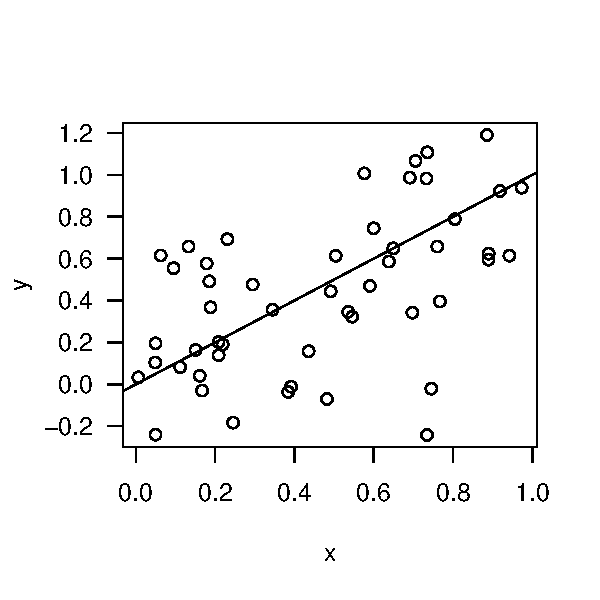
\includegraphics[width=\textwidth]{figs/myfigure.pdf}
    
%\vspace{-2em}
    
%\caption{Figure placement is a dificult in this template.}
%\label{fig:myfigure}
        
%\end{framed}
%\vspace{-2em}
%\end{wrapfigure}
 

% to reference figures and tables use: (\textbf{\textit{Fig.~\ref{}}})




% do not number pages for submission, but useful for drafts.
%\pagenumbering{arabic} 
\begin{document}

%\textbf{RESEARCH APPROACH}

\section{Significance}

Cite with {\texttt \textbackslash autocite\{\}}\autocite{Wilson2017}.


\begin{wrapfigure}{r}{.44\textwidth}

\vspace{-3.25em}
\begin{framed}

\vspace{-3em}

\centering
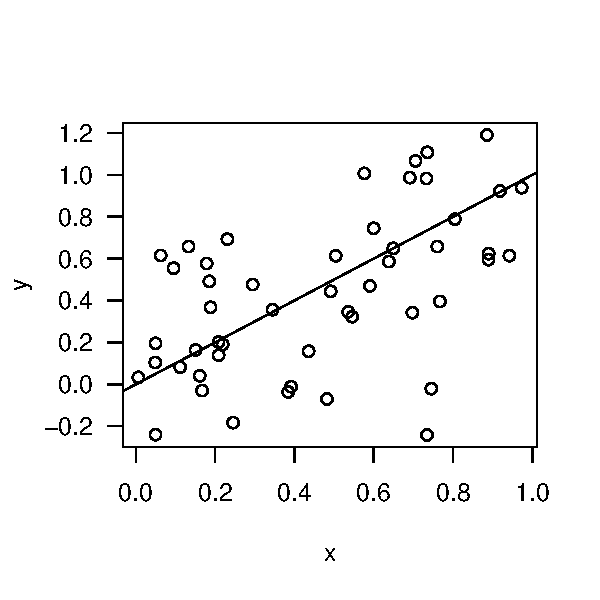
\includegraphics[width=\textwidth]{figs/myfigure.pdf}
    
\vspace{-2em}
    
\caption{Figure placement is a pain in this template.}
\label{fig:myfigure}
        
\end{framed}
\vspace{-2em}
\end{wrapfigure}

\lipsum[2-4]



\section{Innovation}



\section{Approach}

\subsection{Aim 1: ...}






\end{document}

